%%%%%%%%%%%%%%%%%%%%%%%%%%%%%%%%%%%%%%%%%
% Short Sectioned Assignment
% LaTeX Template
% Version 1.0 (5/5/12)
%
% This template has been downloaded from:
% http://www.LaTeXTemplates.com
%
% Original author:
% Frits Wenneker (http://www.howtotex.com)
%
% License:
% CC BY-NC-SA 3.0 (http://creativecommons.org/licenses/by-nc-sa/3.0/)
%
%%%%%%%%%%%%%%%%%%%%%%%%%%%%%%%%%%%%%%%%%

%----------------------------------------------------------------------------------------
%	PACKAGES AND OTHER DOCUMENT CONFIGURATIONS
%----------------------------------------------------------------------------------------

\documentclass[paper=a4, fontsize=11pt]{scrartcl} % A4 paper and 11pt font size

\usepackage[T1]{fontenc} % Use 8-bit encoding that has 256 glyphs
\usepackage{fourier} % Use the Adobe Utopia font for the document - comment this line to return to the LaTeX default
\usepackage[spanish]{babel} % English language/hyphenation
\selectlanguage{spanish}
\usepackage[utf8]{inputenc}
\usepackage{amsmath,amsfonts,amsthm} % Math packages
\usepackage{graphicx}

\usepackage{sectsty} % Allows customizing section commands
\allsectionsfont{\centering \normalfont\scshape} % Make all sections centered, the default font and small caps

\usepackage{fancyhdr} % Custom headers and footers
\pagestyle{fancyplain} % Makes all pages in the document conform to the custom headers and footers
\date{}
\fancyhead{} % No page header - if you want one, create it in the same way as the footers below
\fancyfoot[L]{} % Empty left footer
\fancyfoot[C]{} % Empty center footer
\fancyfoot[R]{\thepage} % Page numbering for right footer
\renewcommand{\headrulewidth}{0pt} % Remove header underlines
\renewcommand{\footrulewidth}{0pt} % Remove footer underlines
\setlength{\headheight}{5.6pt} % Customize the height of the header

\numberwithin{equation}{section} % Number equations within sections (i.e. 1.1, 1.2, 2.1, 2.2 instead of 1, 2, 3, 4)
\numberwithin{figure}{section} % Number figures within sections (i.e. 1.1, 1.2, 2.1, 2.2 instead of 1, 2, 3, 4)
\numberwithin{table}{section} % Number tables within sections (i.e. 1.1, 1.2, 2.1, 2.2 instead of 1, 2, 3, 4)

\setlength\parindent{0pt} % Removes all indentation from paragraphs - comment this line for an assignment with lots of text

%----------------------------------------------------------------------------------------
%	TITLE SECTION
%----------------------------------------------------------------------------------------

\newcommand{\horrule}[1]{\rule{\linewidth}{#1}} % Create horizontal rule command with 1 argument of height

\title{	
\normalfont \normalsize 
\textsc{UNIVERSIDAD DE CANTABRIA, DEPARTAMENTO DE FÍSICA MODERNA} \\ [20pt] % Your university, school and/or department name(s)
\horrule{0.5pt} \\[0.4cm] % Thin top horizontal rule
\huge Física de Partículas Elementales (G71) \\ % The assignment title
\normalsize 4 Curso - Grado de Física - Doble Grado Física Matemáticas - Ejercicios Tema 6
\horrule{2pt} \\[0.5cm] % Thick bottom horizontal rule
}

\begin{document}

\maketitle % Print the title

\vspace{-2.5cm}

%----------------------------------------------------------------------------------------
%	PROBLEM 1
%----------------------------------------------------------------------------------------
\textbf{Cuestión 1.} Madame Wu diseñó un experimento en el que un núcleo de cobalto decae en un núcleo de
níquel, un electrón y un antineutrino: Co~$\rightarrow$~Ni + e$^{-}$ + $\nu$ en presencia de un campo magnético. El diagrama
mostrado a continuación contiene un esquema de este proceso para dos situaciones en las que el campo magnético está alineado
(derecha) o antialineado (izquierda) con el eje Z. En ambos casos el spin del cobalto y del níquel se alinea siguiendo el campo magnético. Puesto
que el níquel tiene una unidad menos de spin que el cobalto, el electrón y el anti-neutrino tendrán que compensar la pérdida de spin tal
y como se indica en el diagrama. Asigna y calcula los espinores de Dirac autoestados de la helicidad a cada uno de los electrones y antineutrinos en el
diagrama, en función del momento p y las masas (asume $\phi$ = 0). Asumiendo que la masa del neutrino es exactamente 0, uno de los diagramas tiene
una probabilidad de ocurrir igual a 0. Indica cuál y explica por qué en relación al elemento de matriz asociado a la fuerza débil mediada por un
bosón W. Usando los espinores de Dirac y los operadores de proyección quiral demuestra lo mismo matemáticamente. 

\begin{figure}[!h]
\begin{center}
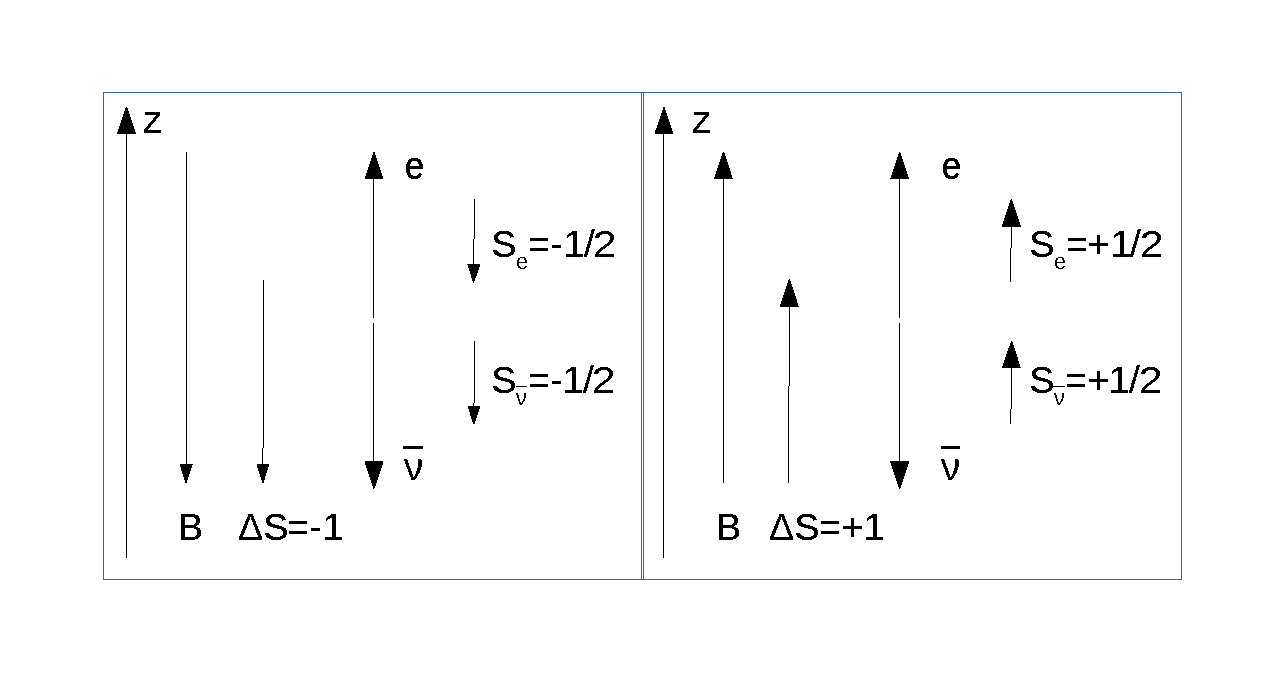
\includegraphics[width=0.6\linewidth]{DibujoExamen.pdf}
\end{center}
\end{figure}

%----------------------------------------------------------------------------------------
%       PROBLEM 2
%----------------------------------------------------------------------------------------
\textbf{Cuestión 2.} Calcula las componentes quirales right y left de los dos espinores de partícula y antípartícula con helicidad positiva y negativa. Demuestra que en el límite de masa nula las
componentes left-handed de antipartícula y las componentes right-handed de partícula se anulan.
\\
\\
  





\end{document}
